\def\year{2015}
%File: formatting-instruction.tex
\documentclass[letterpaper]{article}
\usepackage{aaai}
\usepackage{times}
\usepackage{helvet}
\usepackage{courier}
\usepackage{graphicx}
\usepackage{subcaption}
\usepackage{}
\frenchspacing
\setlength{\pdfpagewidth}{8.5in}
\setlength{\pdfpageheight}{11in}
\pdfinfo{
/Title (Insert Your Title Here)
/Author (Put All Your Authors Here, Separated by Commas)}
\setcounter{secnumdepth}{1}  
 \begin{document}
% The file aaai.sty is the style file for AAAI Press 
% proceedings, working notes, and technical reports.
%
\title{Combining Learning and Evolution in OpenNERO}
\author{Jacob Robertson \and Yun Wu\\
Department of Computer Science\\
University of Texas at Austin\\
}
\maketitle
\begin{abstract}
\begin{quote}
AAAI
\end{quote}
\end{abstract}

\section{Experiments and Results}
\label{sec:exp}
In this paper, we evaluated our rtNEAT+Q algorithm in OpenNERO\footnote{https://code.google.com/p/opennero/}. OpenNERO is an open source software platform designed for research and education in Artificial Intelligence. The project is based on the Neuro-Evolving Robotic Operatives (NERO) game developed by graduate and undergraduate students at the Neural Networks Research Group and Department of Computer Science at the University of Texas at Austin. In the NERO game, The learning agents in NERO are simulated robots, and the goal is to train a team of these agents for combat. The agents begin the game with no skills and only the ability to learn. As shown in Figure~\ref{fig:opennero}, in this project we focus on the task of approaching a flag in different scenarios.
\begin{figure}[ht]
\centering
  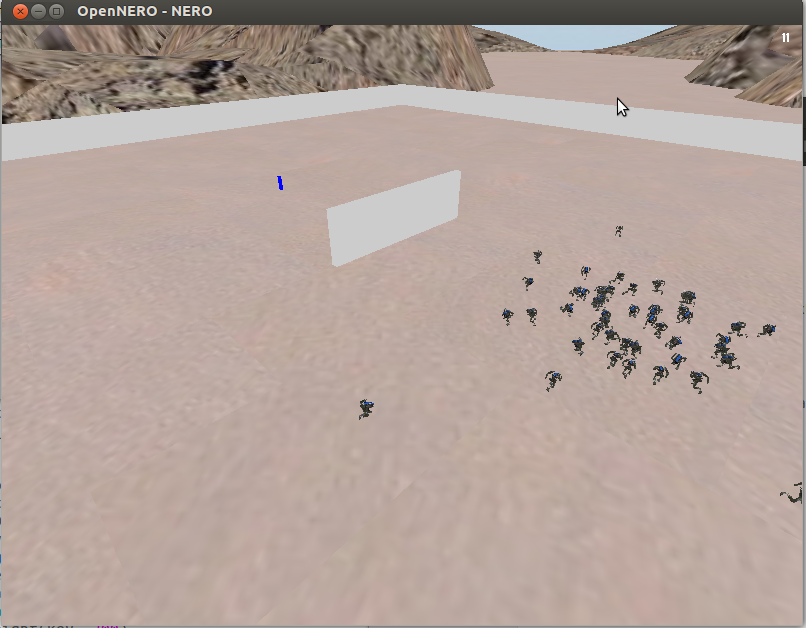
\includegraphics[width=0.7\columnwidth]{opennero.png}
\caption{OpenNERO scenario}
\label{fig:opennero}
\end{figure}

\subsection{Approaching a flag}
The first task is to run towards a flag directly. The distance between the spawn spot of agents and the flag is 141.4. Figure~\ref{fig:flag} illustrates the result. The green line is the average distance among all the agents and the blue line shows the change of the minimum distance. From Figure~\ref{fig:flag_q} we can find that the result of Q learning in continuous domain is quite unstable. rtNEAT, however, performs much better. The most fast agent gets to the flag quickly (around 25 ticks). The average distance converges at around 200 ticks when most agents has learnt to approach a flag. The combination of rtNEAT and Q learning has similar performance with rtNEAT. The average distance converges quickly but is longer than the rtNEAT agents. 
\begin{figure*}[ht]
\centering
\begin{subfigure}{0.7\columnwidth}
  \centering
  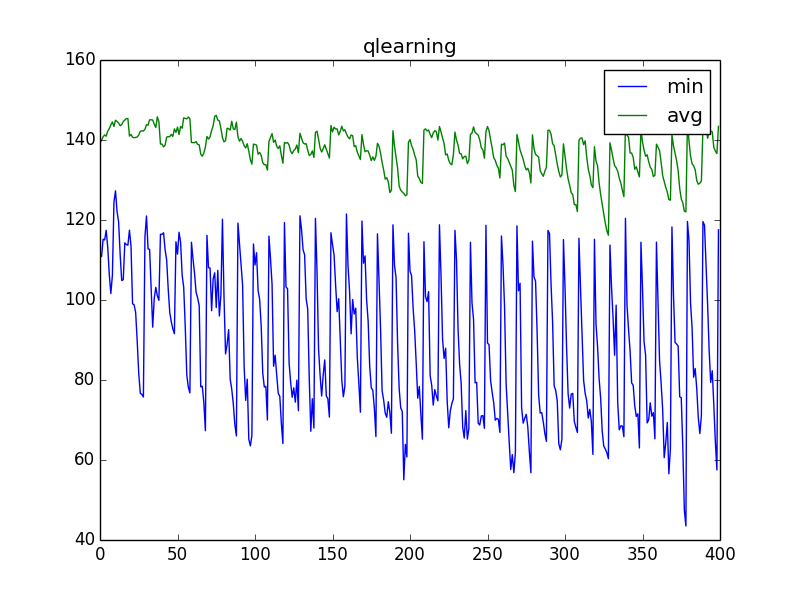
\includegraphics[width=\columnwidth]{flag_qlearning.png}
  \caption{Q Learning}
  \label{fig:flag_q}
\end{subfigure}%
\begin{subfigure}{0.7\columnwidth}
  \centering
  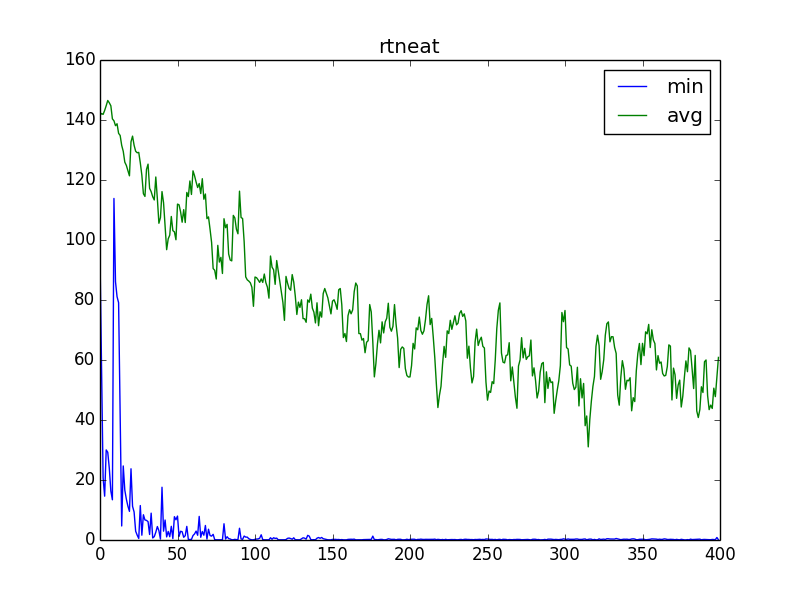
\includegraphics[width=\columnwidth]{flag_rtneat.png}
  \caption{rtNEAT}
  \label{fig:flag_neat}
\end{subfigure}
\begin{subfigure}{0.7\columnwidth}
  \centering
  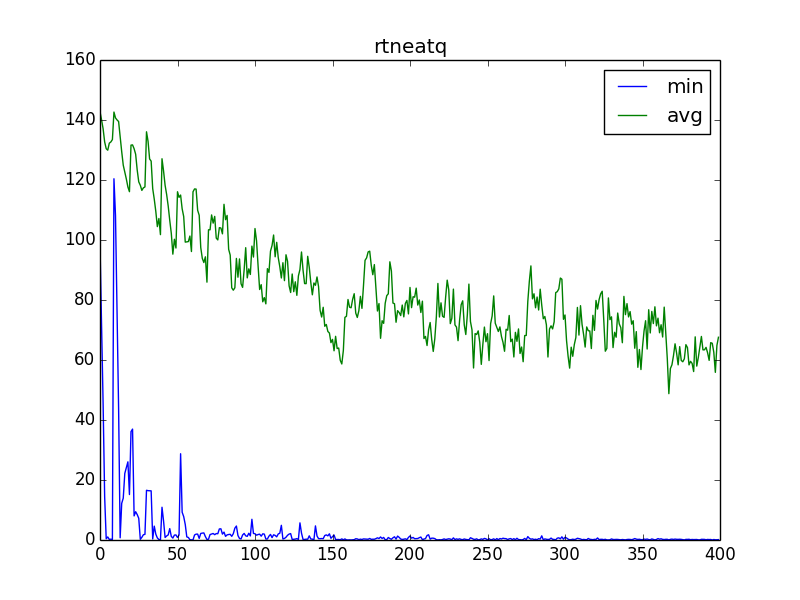
\includegraphics[width=\columnwidth]{flag_rtneatq.png}
  \caption{rtNEAT + Q Learning}
  \label{fig:flag_neatq}
\end{subfigure}
\caption{Approaching a flag}
\label{fig:flag}
\end{figure*}

\subsection{Approaching a moving flag}
We also experimented on approaching a moving flag with different algorithms(Figure~\ref{fig:moving}). Here, the location of the flag is updated randomly every 50 ticks. The minimum distance is 141 and the maximum is 283. For all three algorithm, the process of location update is the same. rtNEAT agents are able to run towards the flag within the first 50 ticks. And after every update, both minimum distance and average distance drop dramatically. The combination of rtNEAT and Q learning is able to learn the behavior within first three updates. And the average distance after 50 ticks is also longer than rtNEAT alone, which is consistent with static flag. The performance of Q learning is still unsatisfactory. The average distance does not change much after long time of training.

\begin{figure*}[ht]
\centering
\begin{subfigure}{0.7\columnwidth}
  \centering
  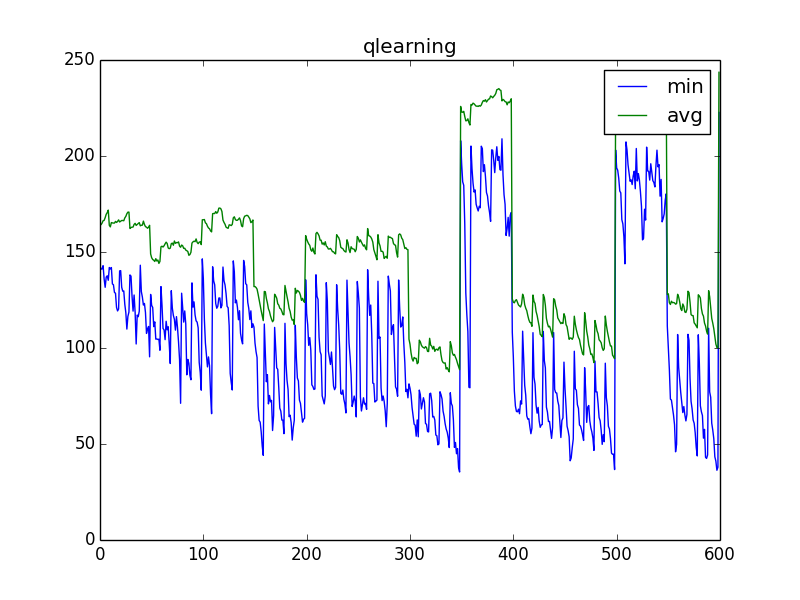
\includegraphics[width=\columnwidth]{moving_qlearning.png}
  \caption{Q Learning}
  \label{fig:moving_q}
\end{subfigure}%
\begin{subfigure}{0.7\columnwidth}
  \centering
  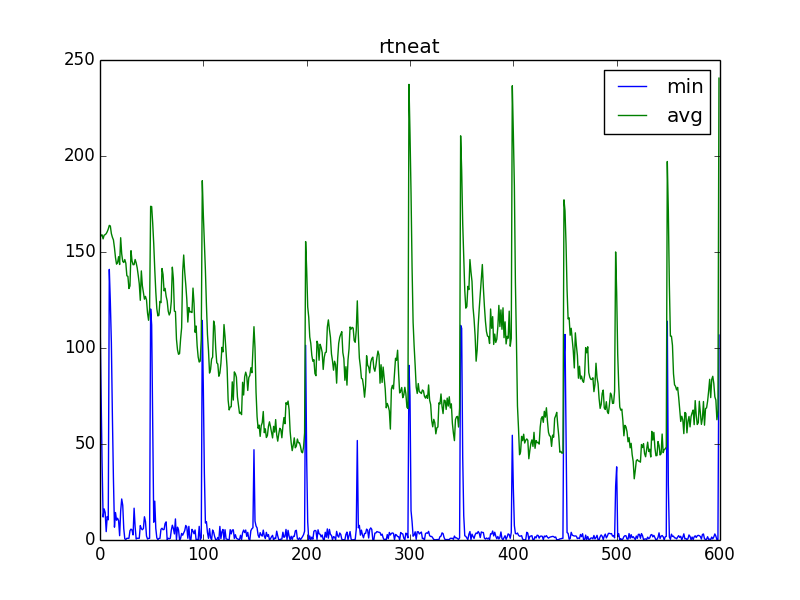
\includegraphics[width=\columnwidth]{moving_rtneat.png}
  \caption{rtNEAT}
  \label{fig:moving_neat}
\end{subfigure}
\begin{subfigure}{0.7\columnwidth}
  \centering
  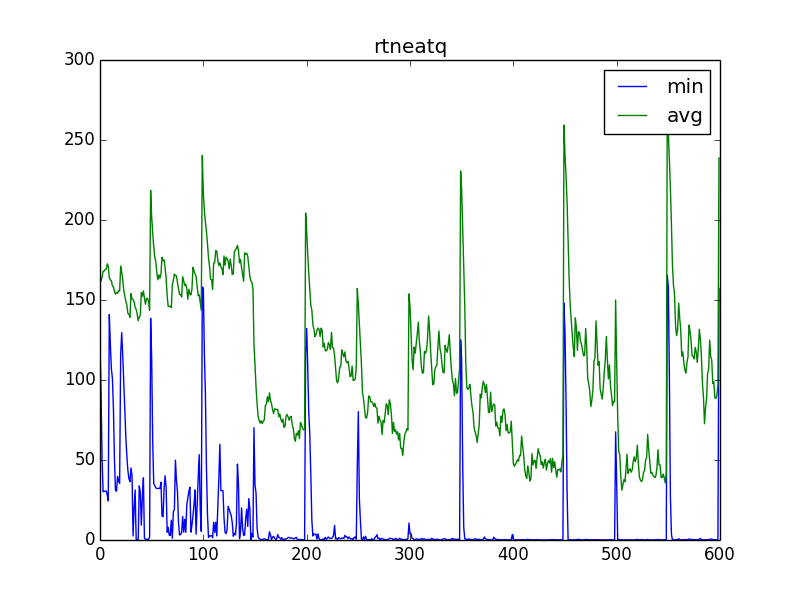
\includegraphics[width=\columnwidth]{moving_rtneatq.png}
  \caption{rtNEAT + Q Learning}
  \label{fig:moving_neatq}
\end{subfigure}
\caption{Approaching a moving flag}
\label{fig:moving}
\end{figure*}


\subsection{Approaching a flag with obstacles}
However, when it comes to more complex tasks, the benefit of learning appears. In the third experiments, the distance between agents and the flag is 267. And there is a wall with width 100 between them. Agents need to learn to get around the wall to approach the flag. As shown in Figure~\ref{fig:wall}, Q learning agents never get a chance to get close to the flag within 700 ticks. The minimum distance between agents and flag is about 170. However, from Figure~\ref{fig:wall_neat} and Figure~\ref{fig:wall_neatq}, it is clear that at first, agents learn to go directly towards flag until they are blocked by the wall. Then exploration then helps find the way around. Q learning then back propagate their network and learn the route. Finally, although rtNEAT+Q converges more slowly than rtNEAT, agents runs toward the flag more fast. The average distance of rtNEAT converges to 180 while that of rtNEAT+Q to 150. 
\begin{figure*}[ht]
\centering
\begin{subfigure}{0.7\columnwidth}
  \centering
  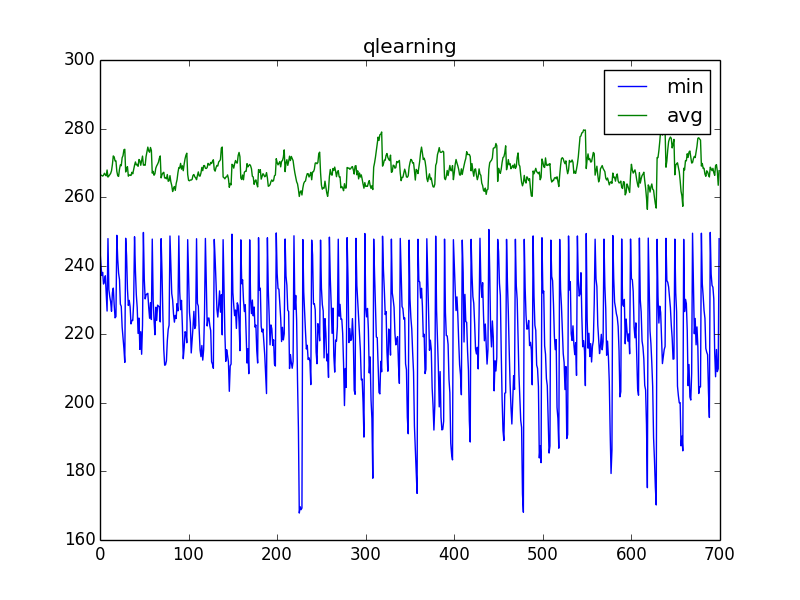
\includegraphics[width=\columnwidth]{wall_qlearning.png}
  \caption{Q Learning}
  \label{fig:wall_q}
\end{subfigure}%
\begin{subfigure}{0.7\columnwidth}
  \centering
  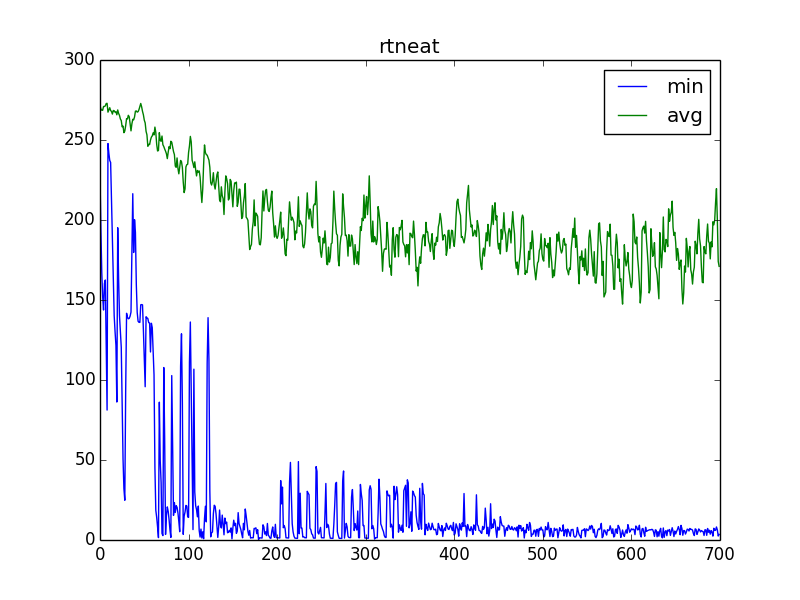
\includegraphics[width=\columnwidth]{wall_rtneat.png}
  \caption{rtNEAT}
  \label{fig:wall_neat}
\end{subfigure}
\begin{subfigure}{0.7\columnwidth}
  \centering
  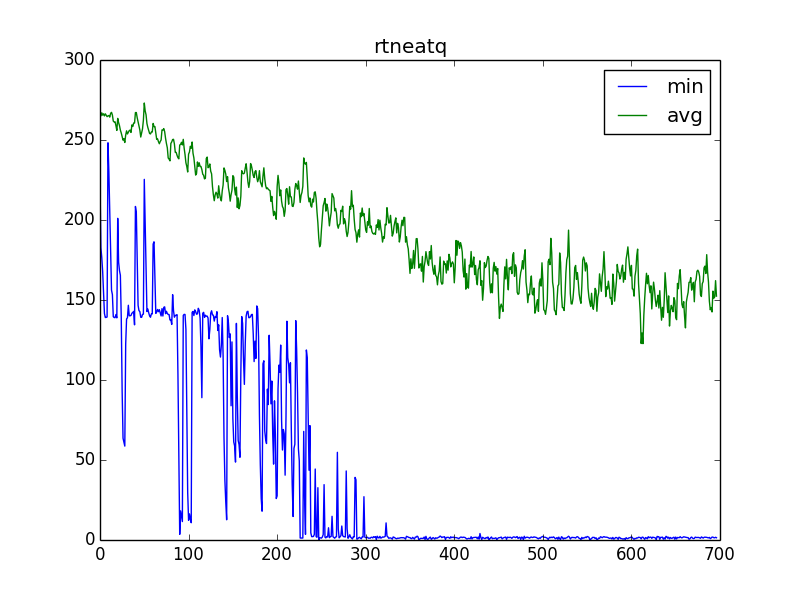
\includegraphics[width=\columnwidth]{wall_rtneatq.png}
  \caption{rtNEAT + Q Learning}
  \label{fig:wall_neatq}
\end{subfigure}
\caption{Approaching a flag with obstacles}
\label{fig:wall}
\end{figure*}

\section{Discussion and Future Work}
The results presented in Section~\ref{sec:exp}, demonstrate the performance of combination of rtNEAT and Q learning. It shows that the performance is related to the complexity of the task. Intuitively, evolution can help develop ability to survive by coding into the genomes, like breathing and metabolism. Such mechanism is relatively simple. Also, it requires little calculation with changing environment. Therefore, such ability can be developed by evolution alone. On the other hand, scientific knowledge or etiquette are examples of complicated tasks for humans. A proper reaction to different situations in social life is intricate and requires large computation and memory search. In those cases, learning within a lifetime of a generation is more effective than relying on evolution itself. Similarly, in our experiments, approaching a flag is relatively simple. Thus evolution itself can build up an accurate neural network. However, it is not straightforward how to get to a flag with an obstacle in the way. Agents need to learn to go away from the flag to get around the wall. There are different paths and learning could also help us find the shortest one.

Here is the reason why rtNEAT+Q benefits complex tasks. rtNEAT+Q takes advantage of TD updates to tune parameters of neural network. However, Q learning needs time to learn. In simple task, structure of neural network is relatively simple. rtNEAT itself is able to evolve the optimal method quickly. However, for complicated tasks, it takes more time for evolution. In the mean time, Q learning is able to back propagate the network based on TD updates. Lamarckian system is used in our implementation, where the result of learning is kept to the next generation. 

According to our result, rtNEAT+Q can successfully train neural network function approximators. However, rtNEAT+Q requires many more episodes to find good solutions than rtNEAT do in the same domain. Since each candidate network must be trained long enough to let Q-learning work, it has very high sample complexity. Moreover, for each episode, rtNEAT+Q also takes around 40\% more time than rtNEAT. The extra time is used to back propagate neural networks according to TD updates. However, such process is independent of the policy the agent is following, one network can be updated while another is controlling the agent. Furthermore, a network can be updated based on data saved from previous sample episodes, regardless of what policy was used during those episodes. Consequently,
it is not necessary to use different episodes to train each network. As shown in \cite{whiteson2006sample}, we could save data from the episodes used by the previous generation, each network in the population can be pre-trained off-line

Also, Figure~\ref{fig:flag}-~\ref{fig:wall} show that Q learning does not perform well in our experiments. It is always a challenge for reinforcement learning in continuous domain. The implementation there is simply discretization the orientation to lots of intervals. It will cause a huge search space. Thus it is difficult to find the optimal solution by TD update. Also, on OpenNERO platform, the lifetime of each agent is related to the fitness to current environment. If the speed of learning is too low, they will be reset and consequently it is difficult for Q learning agents to get to the flag. 

Another problem with Q-learning is the difficulty of exploration. Here, we use $\epsilon$-greedy selection. Each time the agents selects an action, it choose probabilistically between exploration and exploitation. With probability $\epsilon$, it will explore by selecting randomly from the available actions. With probability 1-$\epsilon$, it will exploit by selecting the greedy action. Such mechanism has been proven to provide a balance between exploration and exploitation in discrete domains. However, things are different in continuous domain like OpenNERO. If you pick a random action some small percentage of the time that will just be some little fluctuation in behavior since it will usually be immediately followed by an optimal action. It's like exploration consists of walking just one step off the beaten path instead of taking another path. 

. 

\section{Conclusion}
Reinforcement learning is an appealing and empirically successful approach to finding effective
control policies in large probabilistic domains. There are three ways to solve the problem: evolution, TD update and their combination. Their performances depend on the properties of the task. According to our research and experiments, TD update is more suitable in discrete domains with limited states and actions. Evolution outperforms it in continuous domains and converges quickly in simple tasks. The combination of evolution and TD update can solve complex problems with better result than learning or evolution alone. It takes more time but it also evolves a function approximator during learning. In this project, rtNEAT+Q is implemented for combination of reinforcement learning in continuous domain and realtime evolution. It is tested in OpenNERO to train the agents to approach a flag. The experiments provide insight about the advantages of models related to task complexity.

\section*{Acknowledgements}
Thanks to Professor Risto Miikkulainen for his kind discussion with us about the project. Thanks to Kim Houck for her help with understanding OpenNERO platform.

\bibliographystyle{aaai}
\bibliography{report}



\end{document}
